%!TEX TS-program = xelatex
\documentclass[12pt]{article}

\usepackage[a4paper,top=2.5cm, bottom=2.5cm, left=3cm, right=3cm]{geometry}

\usepackage{fontspec}
\usepackage{xeCJK}
\usepackage{graphicx}
\usepackage{float}
\usepackage{multirow}
\usepackage[dvipsnames]{xcolor}
\usepackage[colorlinks,linkcolor=NavyBlue]{hyperref}
\usepackage{setspace}

\usepackage{caption}
\usepackage{subcaption}

% \usepackage[english]{babel}

\XeTeXlinebreaklocale "zh"
\XeTeXlinebreakskip = 0pt plus 1pt
% \setCJKmainfont{LiHei Pro}
\setCJKmainfont{LiSong Pro}
\newfontfamily{\K}{LiHei Pro}

\newcommand{\todo}[1]{[{\color{red}{#1}}]}
\newcommand{\ci}{$\bigtriangleup$}
\renewcommand{\figurename}{圖}
\renewcommand{\tablename}{表}

% \renewcommand{\baselinestretch}{1.2}

\begin{document}

\begin{center}{Stage-3} ~ {\Huge AlumniBook} ~ {Group-3} \end{center}

\begin{center}
\begin{tabular}{cccc}
郗昀彥 R00725051&郭瀚智 R02725023&鄭立民 R02725041&李奕德 B99705021 \\
張凱涵 B00705027&施淮振 B00705047&倪嘉銘 T02705102&
\end{tabular} 
\vskip .7cm
\noindent\makebox[\linewidth]{\rule{\linewidth}{1pt}}
\end{center}

\tableofcontents

\newpage

%% ############################## %%
%%             Part 1             %%
%% ############################## %%

\begin{center}
\framebox[10cm][c]{Part 1 -- 使用手冊}
\end{center}

\section{系統總覽}

本系統旨在於建構本系所畢業之成員間的聯繫橋梁,加強產學之間的鍵結來使大學成為更珍貴的資產。曾經待過資管系的優秀人才散布在各個不同領域。在超級專業化的現代若能連結正確領域的人來提供系上一些建議與幫助,必能讓資管系所內的課程內容與訓練更加的紮實。所以除了學生間的相互聯絡,本系統也將會提供系友與教授及行政人員進入本系統,對其所擅長之專業領域提供協助。學生亦可藉由本系統盡早深入了解產業現況,獲得更多正確且即時的資訊並對未來發展方向有更確實精確的判斷。

在透過single sign on服務登入本系統後,每個人可以依照自己的習慣決定透露多少資訊,更新基本資料。本系統也會透過single sign on之服務預先幫忙填入一些基本資料,在填入資料後便可以開始方便的使用討論區的功能。

每個人依照個人身分之不同,可能在本系統中找到不同適合自己的服務來達成各自的需求例如同學需要尋找有特定技能的人解惑、學長姐需要找人才系辦人員需要公告新資訊等等不同的需求接可以在本系統中獲得解決。只要在張貼文章時正確的標示文章類別,系統就會發信讓對應於該類別或是正在關注該類別的用戶知道。

本系統旨在於建立一個能夠有效凝聚資管系所內之相關人士,提供一個跨界跨部(研究所與大學部) 之溝通平台。本系統將階段性提供完整的溝通整合服務,冀望成為連結具專業知識的人幫忙解答疑惑,也希望能夠成為校友找人、學生找事之合作橋梁。

\section{使用手冊}

\subsection{登入使用者帳號}
為了順利使用本系統,我們推薦使用者登入來享受完全的服務。請點選右上角的login按鈕(圖一)來透過single sign on 登入本系統。來到登入頁面後請依照指示完成登入步驟。

\begin{figure}[H]
\centering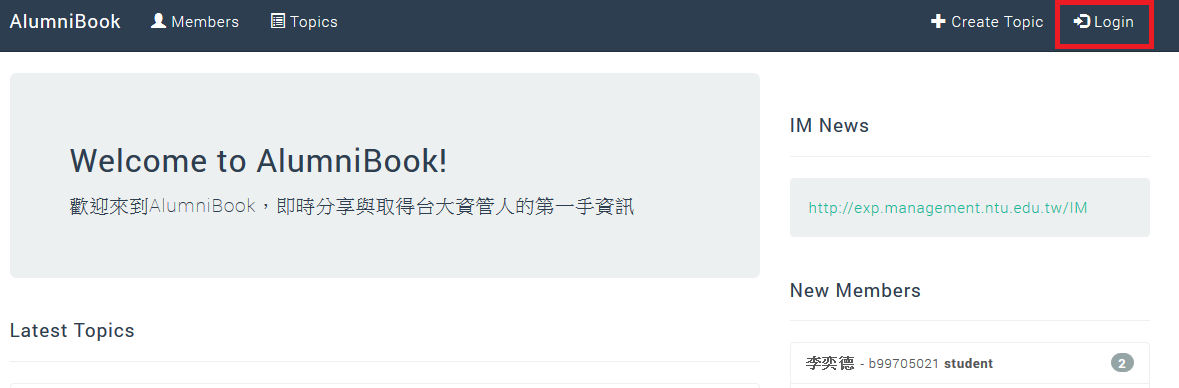
\includegraphics[width=0.7\textwidth]{img/login01.png}
\end{figure}

\subsubsection{以既有帳號登入}
若已有註冊帳號則可在打入帳號密碼後登入系統,否則請聯絡系統管理人員。

\begin{figure}[H]
\centering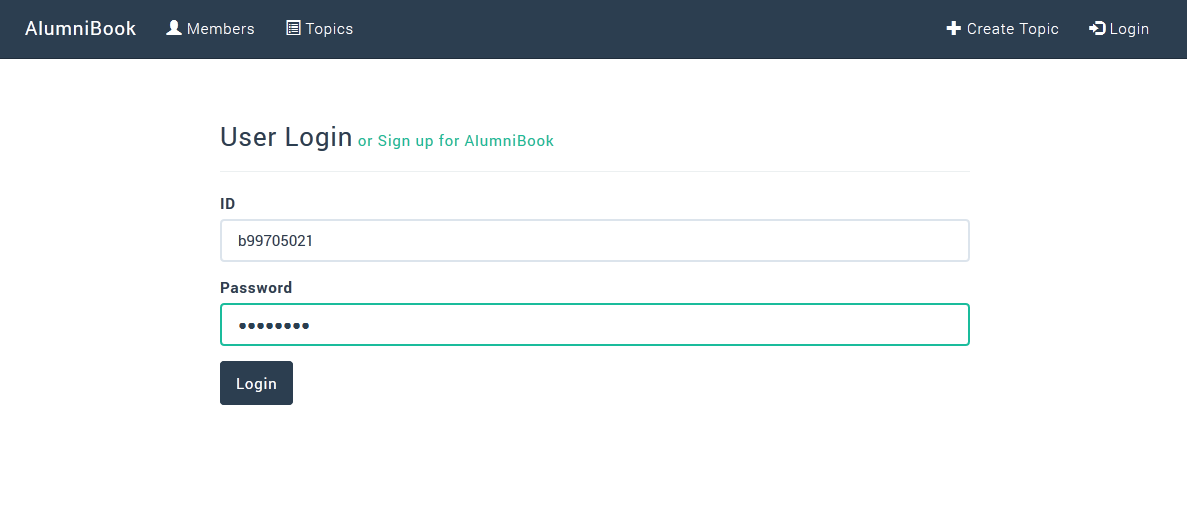
\includegraphics[width=0.7\textwidth]{img/login03.png}
\end{figure}

\subsection{使用者資料設定}
第一次完成登入的使用者會來到自己的資料管理頁面,我們建議使用者填入基本資料來使系統更有效的運作。
\begin{figure}[H]
\centering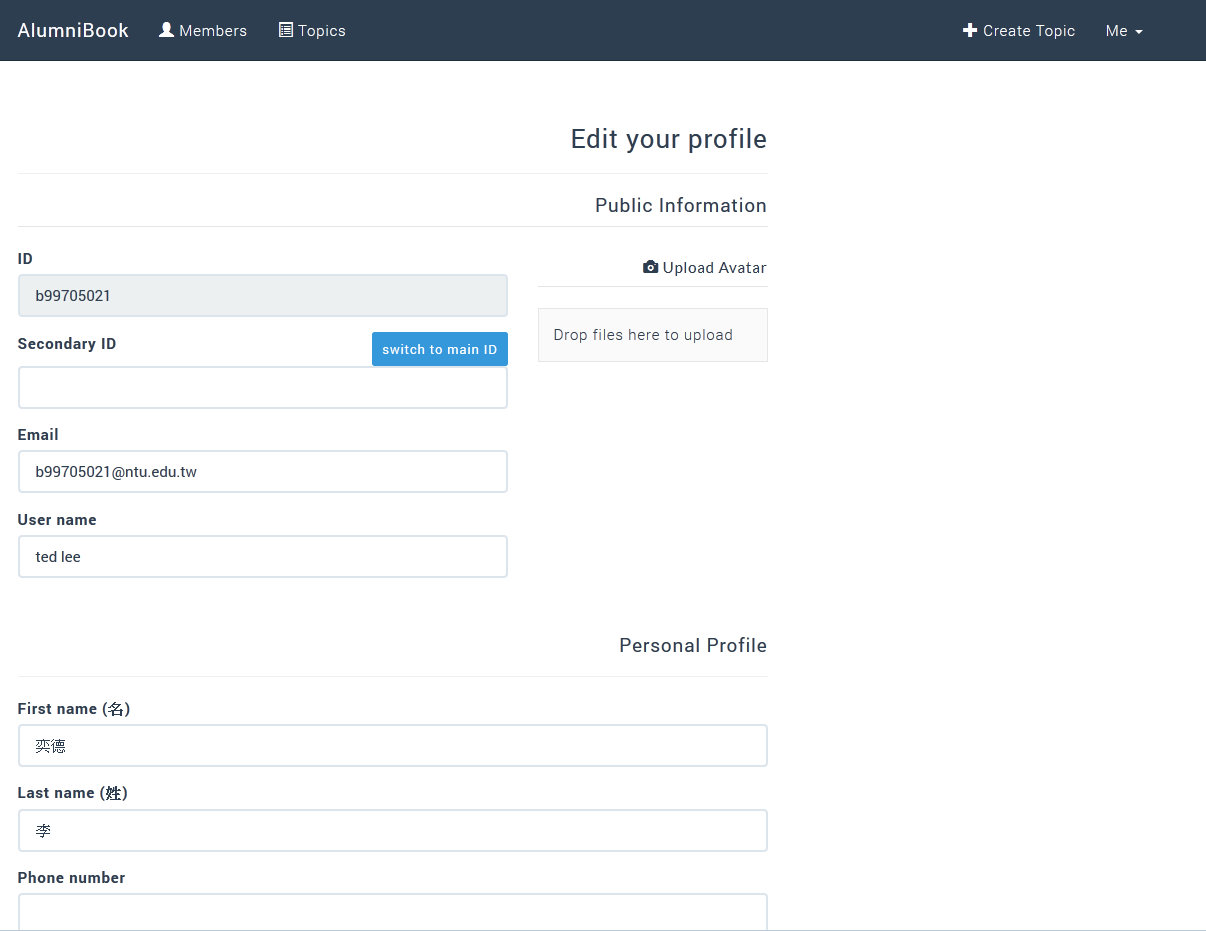
\includegraphics[width=0.7\textwidth]{img/profile01.png}
\end{figure}
不是第一次登入的使用者則可在右上角的me選單中點選profile來修改及增減個人資料的內容。
\begin{figure}[H]
\centering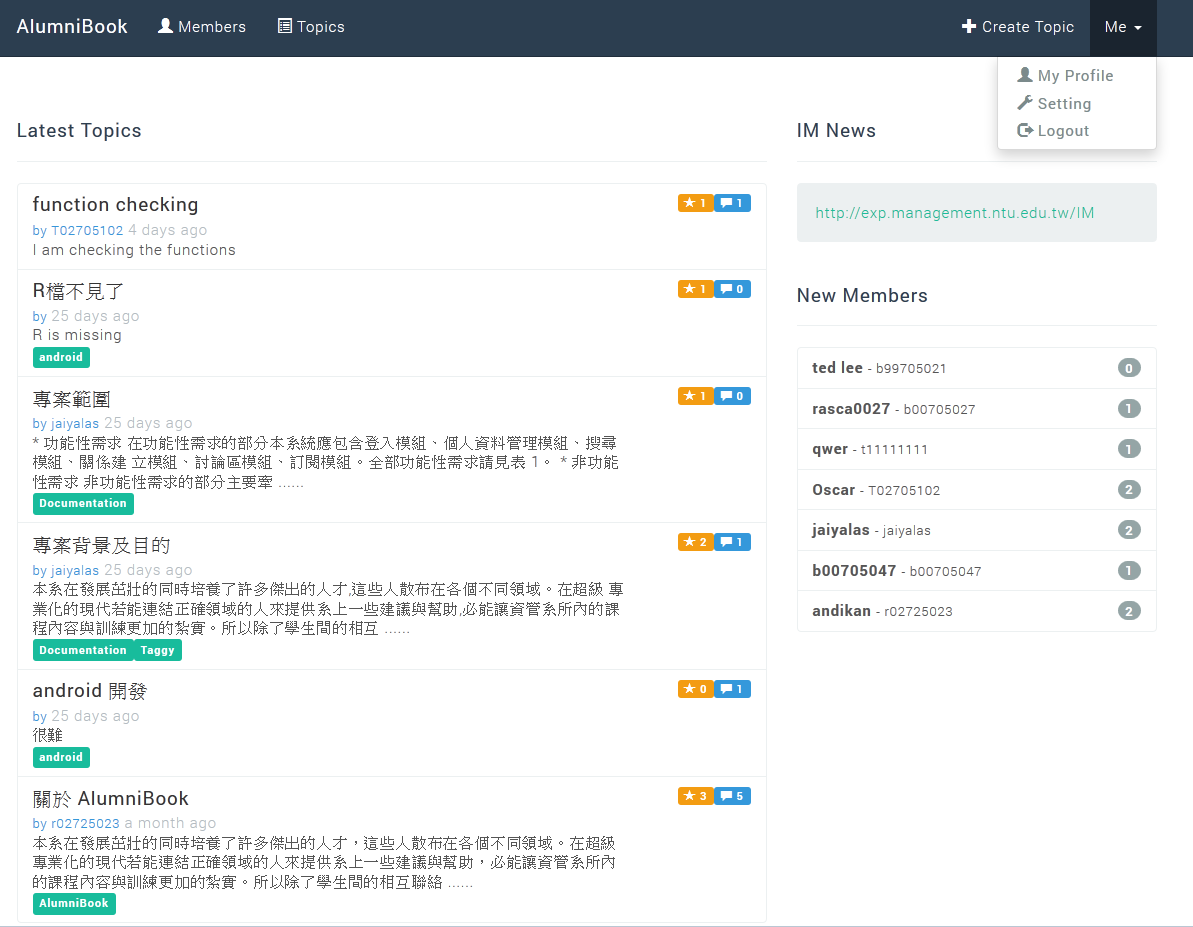
\includegraphics[width=0.7\textwidth]{img/profile02.png}
\end{figure}

\subsection{瀏覽討論區}
不論是否完成登入,使用者皆可以自由的在討論區中流覽各種討論。
\begin{figure}[H]
\centering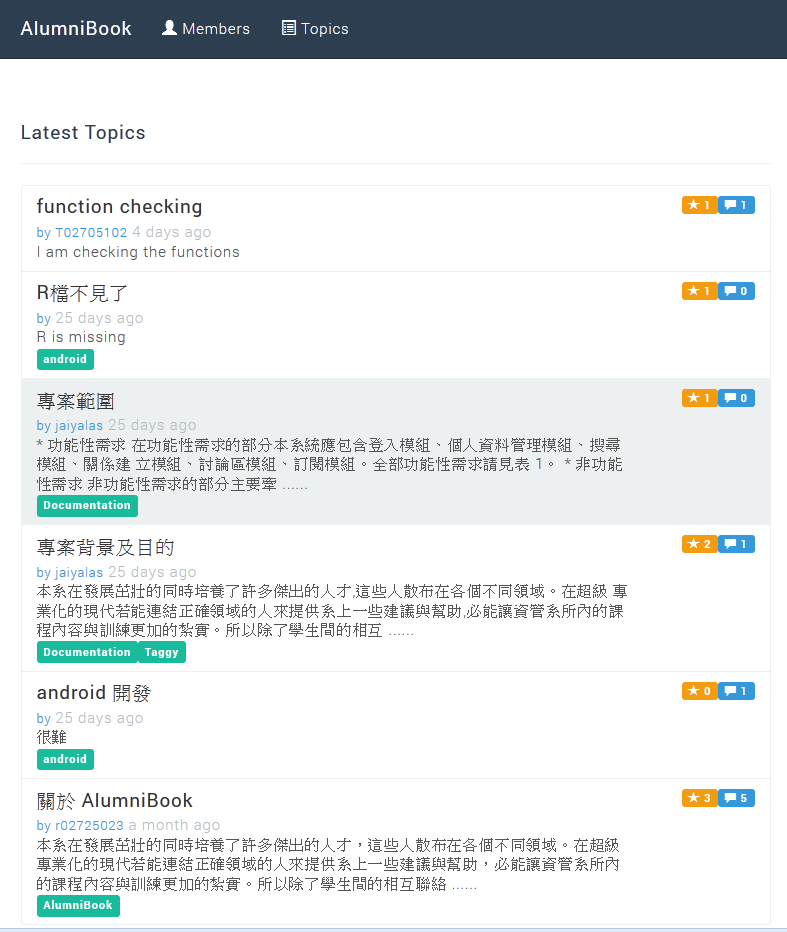
\includegraphics[width=0.7\textwidth]{img/read01.png}
\end{figure}
本系統提供最新的文章列表與所有文章列表,進入本系統之初所見的皆為最新文章列表。

\subsubsection{最新文章列表}
最新文章列表中包含部分的文章,依據時間作為排序規則,顯示固定數量的近期討論。

\subsubsection{所有文章}
所有文章列表中包含本系統中的所有文章。若要進入所有文章列表請點選上方流覽區中間的Topics選項。
\begin{figure}[H]
\centering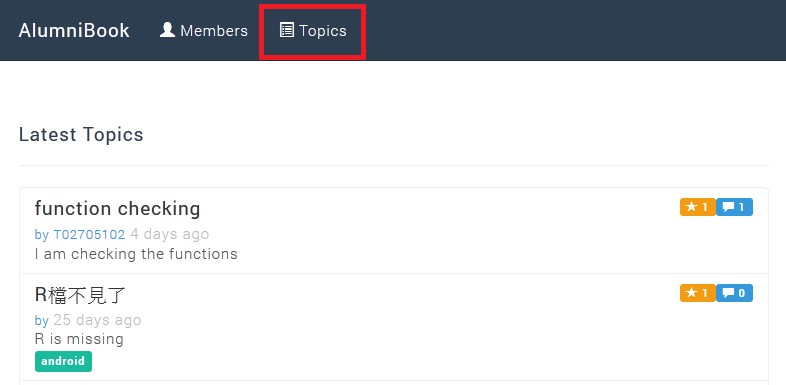
\includegraphics[width=0.7\textwidth]{img/read02.png}
\end{figure}
\begin{figure}[H]
\centering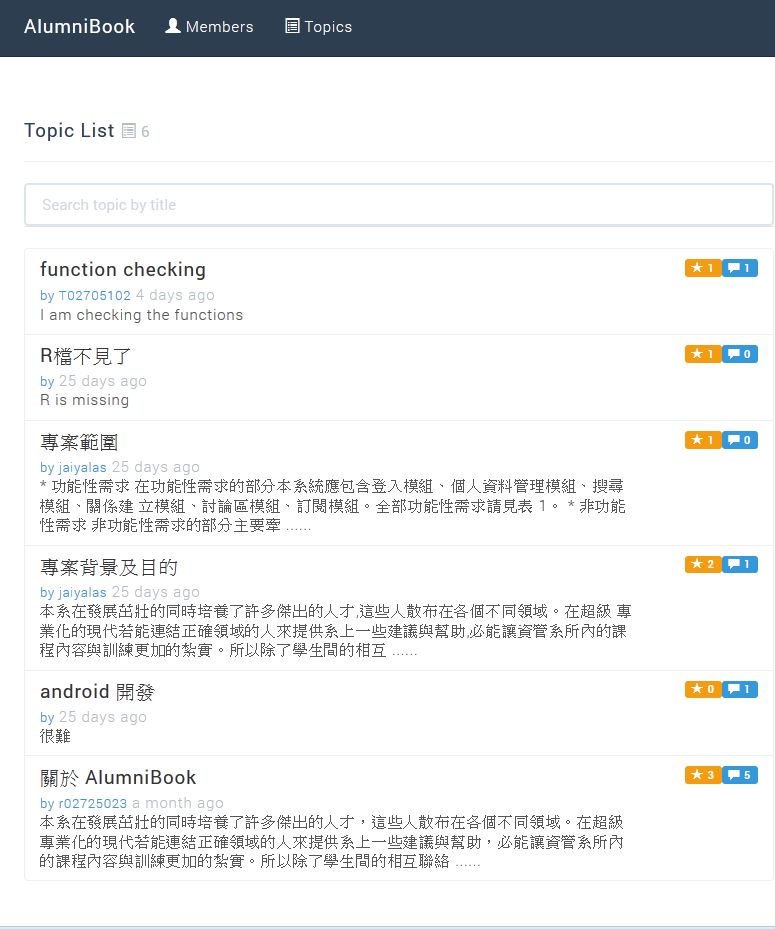
\includegraphics[width=0.7\textwidth]{img/read03.png}
\end{figure}
點選任意的文章後即可在Comments欄位參加討論。
\begin{figure}[H]
\centering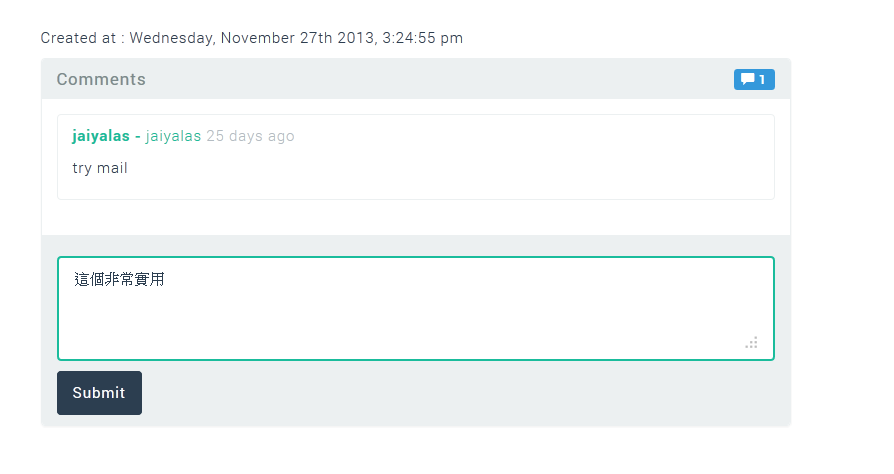
\includegraphics[width=0.7\textwidth]{img/read04.png}
\end{figure}

\subsection{發表文章}
若為以登入使用者則可以在本討論區中撰寫新的文章,本段將簡單介紹撰寫新文章的流程。要發表新文章請點選右上角的+Create Topic來到新增文章的頁面
\begin{figure}[H]
\centering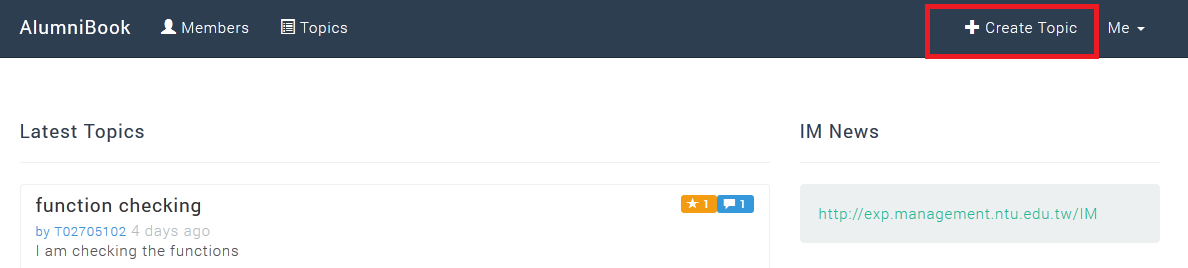
\includegraphics[width=0.7\textwidth]{img/new01.png}
\end{figure}
在各欄位填入資訊後,距離發表文章就不遠了。本系統建議使用者提供文章的分類來讓系統更順暢的運行,只要打上分類名稱後按下add按鈕即可為此文章上標籤,使其他使用者更容易找到這篇文章並了解其內容。
\begin{figure}[H]
\centering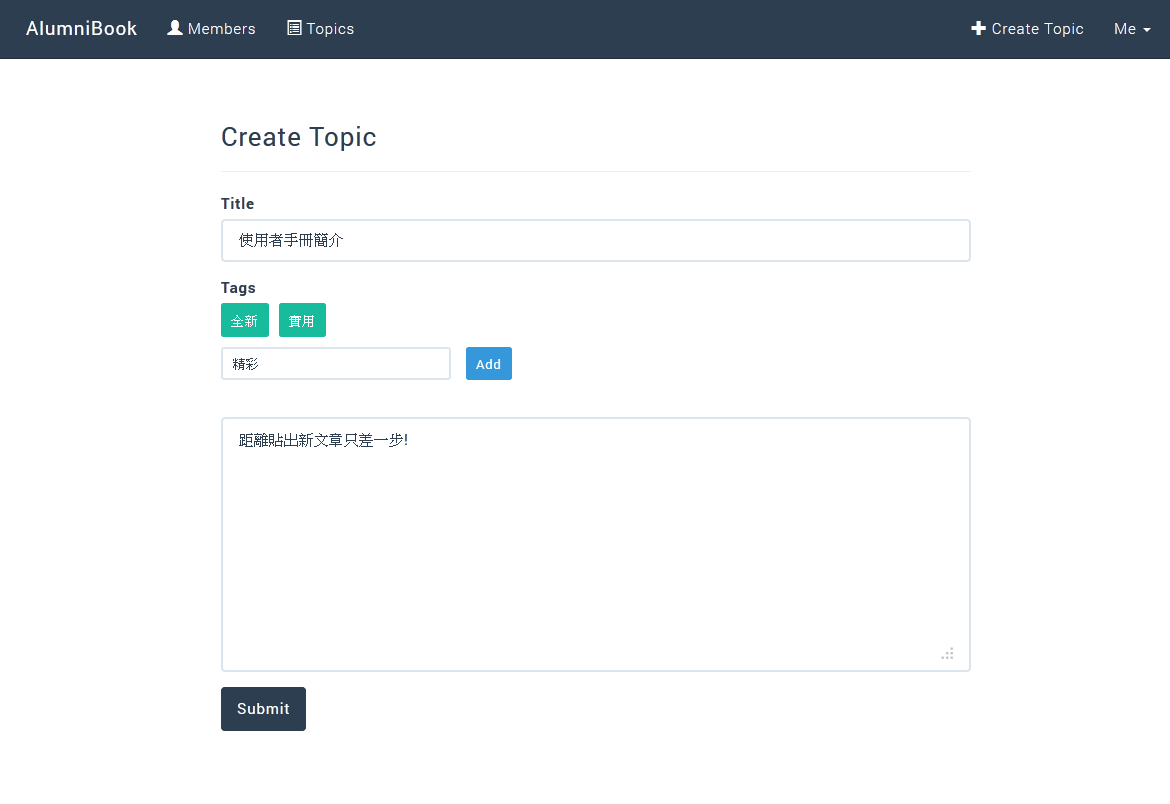
\includegraphics[width=0.7\textwidth]{img/new02.png}
\end{figure}
在按下Submit按鈕後即可將文張貼出於討論看板。
\begin{figure}[H]
\centering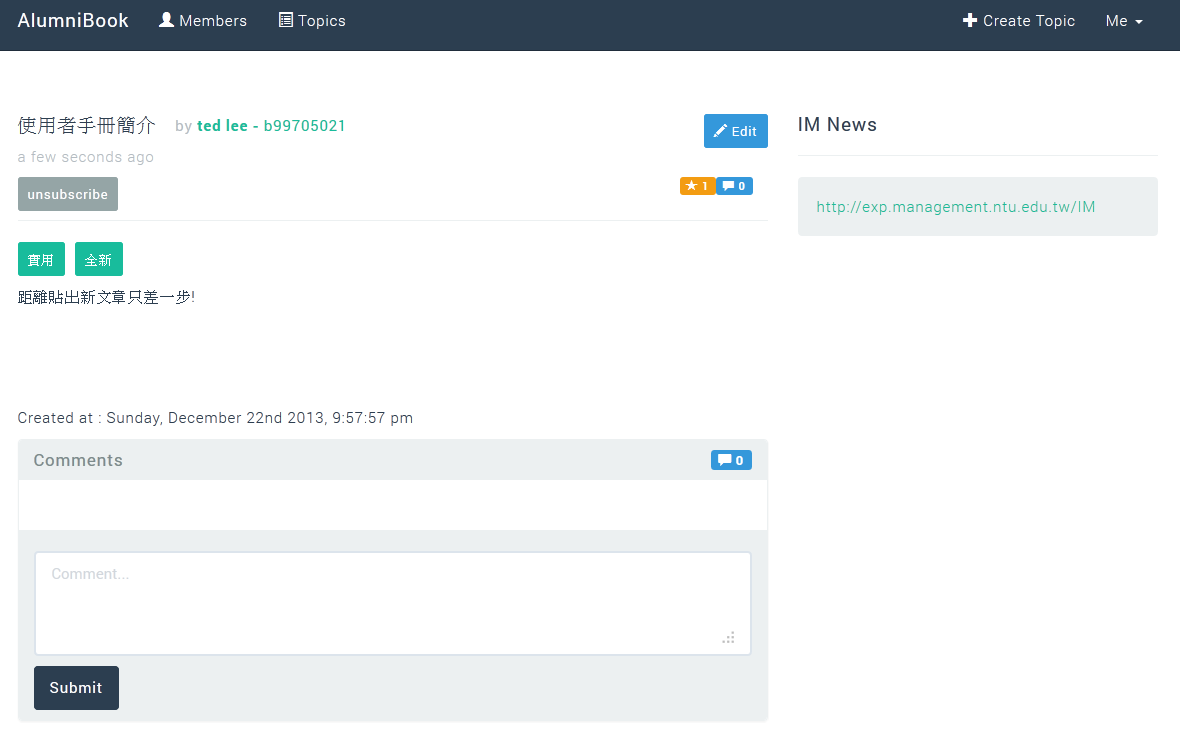
\includegraphics[width=0.7\textwidth]{img/new03.png}
\end{figure}
可在此和其他人交流意見。

\subsection{搜尋使用者}
若在瀏覽過程中對任何人產生興趣,則可點選該名稱即可連結至該用戶的資料頁面。
\begin{figure}[H]
\centering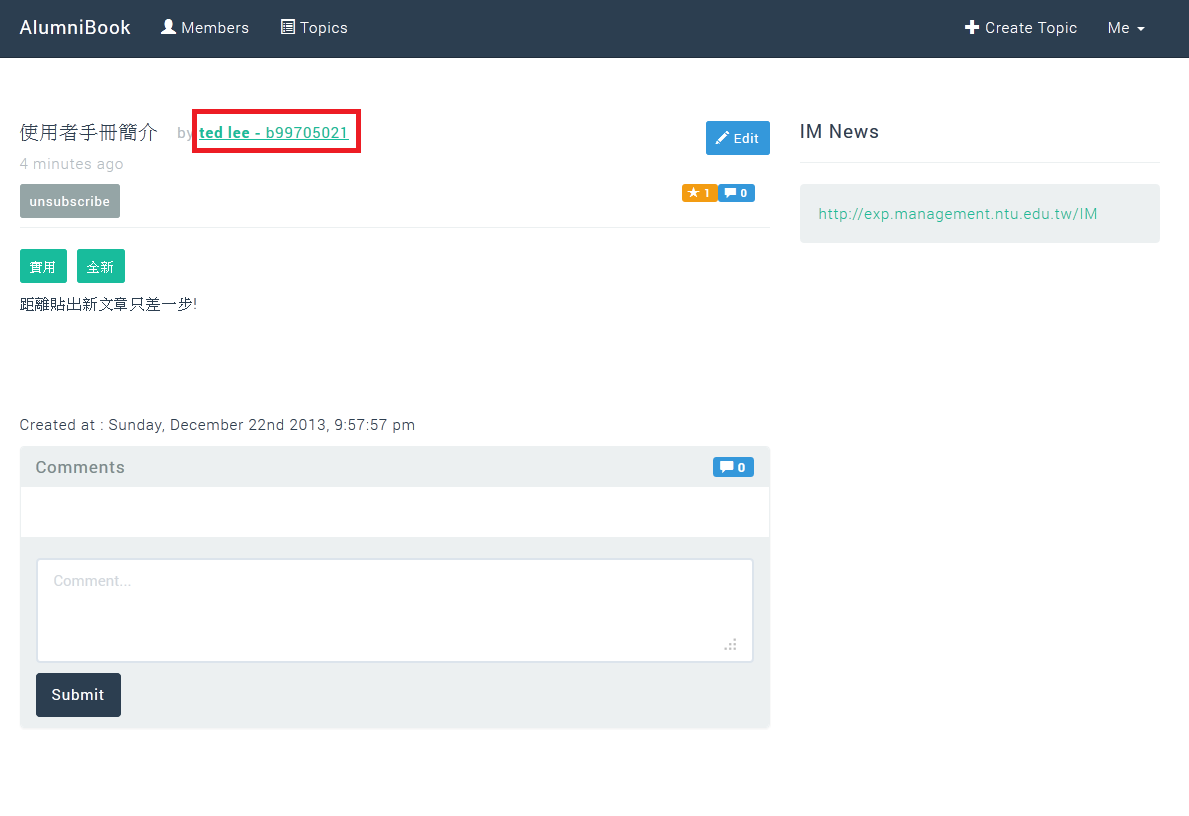
\includegraphics[width=0.7\textwidth]{img/user01.png}
\end{figure}
或是也可以選擇從畫面上端的Members來搜尋,點選Members按鈕後會來到使用者搜尋的頁面。
\begin{figure}[H]
\centering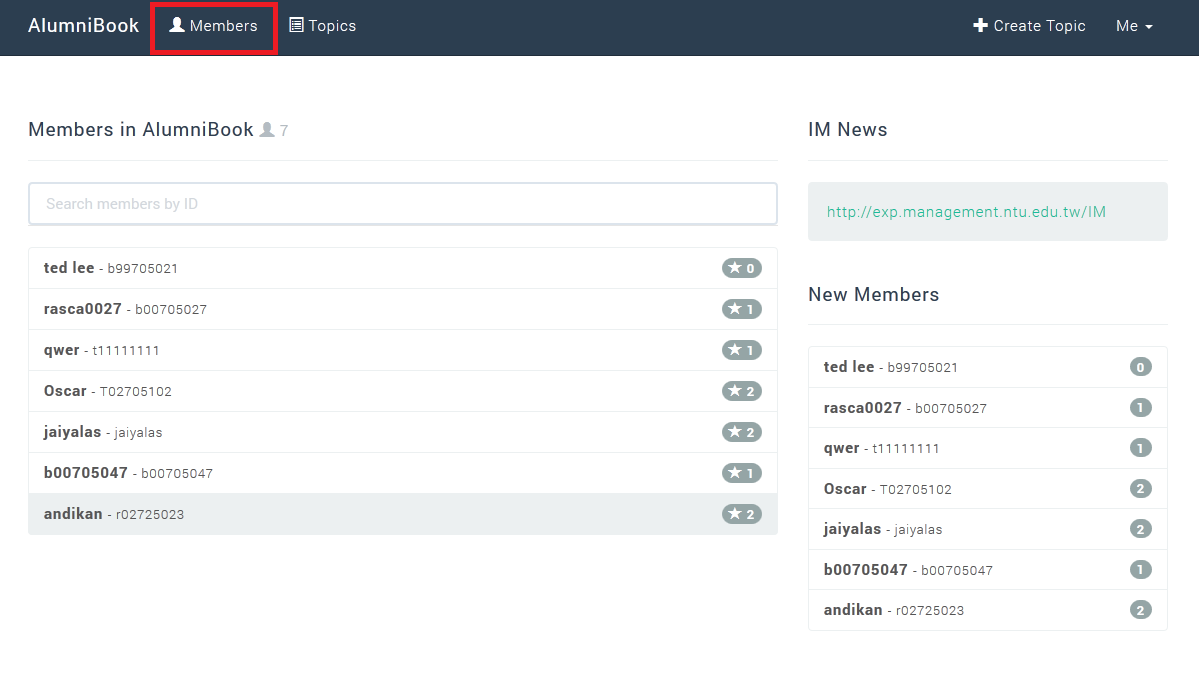
\includegraphics[width=0.7\textwidth]{img/user02.png}
\end{figure}
在搜尋欄位中打入關鍵字後即可找到該用戶,並且造訪他的資料頁面。
\begin{figure}[H]
\centering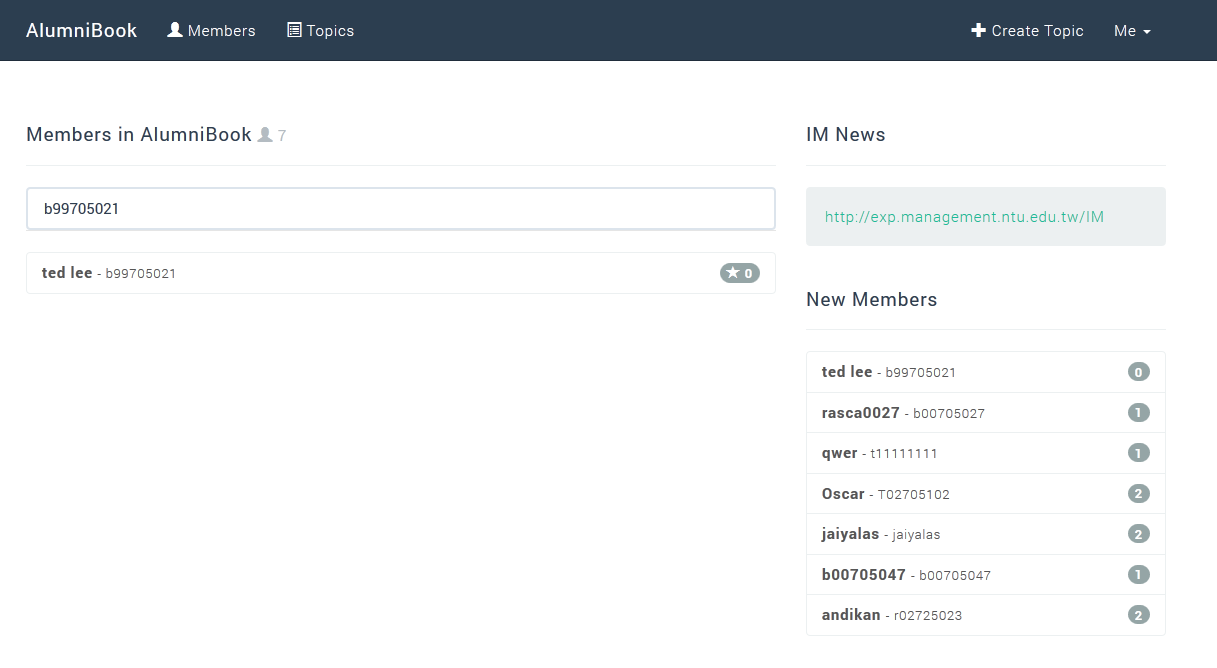
\includegraphics[width=0.7\textwidth]{img/user03.png}
\end{figure}

\subsubsection{追蹤使用者}
若您非常欣賞某位使用者,並且希望在他發布新文章時獲得通知,則可造訪該用戶的資料頁面並且按下Follow。請注意本步驟需在登入之後才可執行。
\begin{figure}[H]
\centering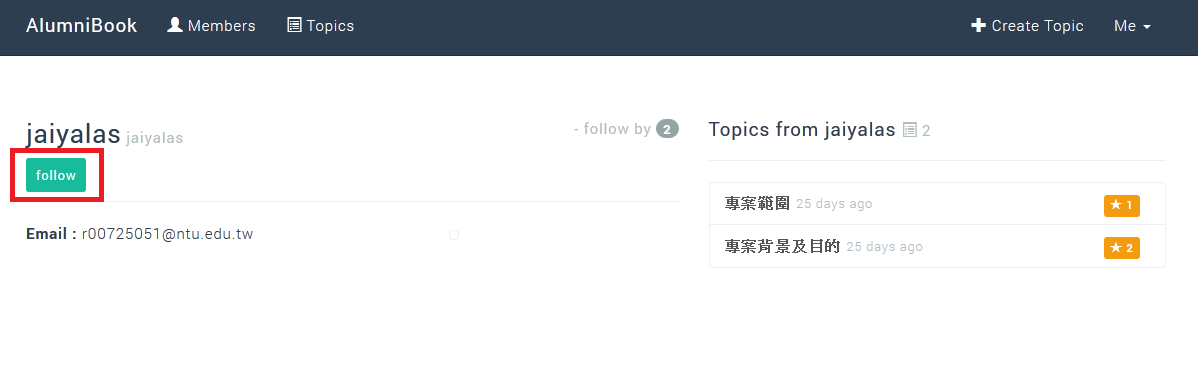
\includegraphics[width=0.7\textwidth]{img/user04.png}
\end{figure}
完成本步驟後每當該用戶發表了新文章時您都會獲得一封通知信,寄至您的學校信箱。

%% ############################## %%
%%             Part 2             %%
%% ############################## %%
\begin{center}
\framebox[10cm][c]{Part 2 -- 專案報告}
\end{center}

\section{專案設計}

\subsection{系統功能}

本系統包含兩個主要的使用情境:「使用者個人資訊與情報的建立與管理」以及「成員之間的互動論壇」。兩者之使用情境如圖~\ref{pic:use:userLogin} 與圖~\ref{pic:use:forum}。實際系統功能之規劃如表~\ref{req} 中所詳列(其中部分沒有實作的功能標示將會標示$^\star$)。

\begin{figure}[H]
\centering
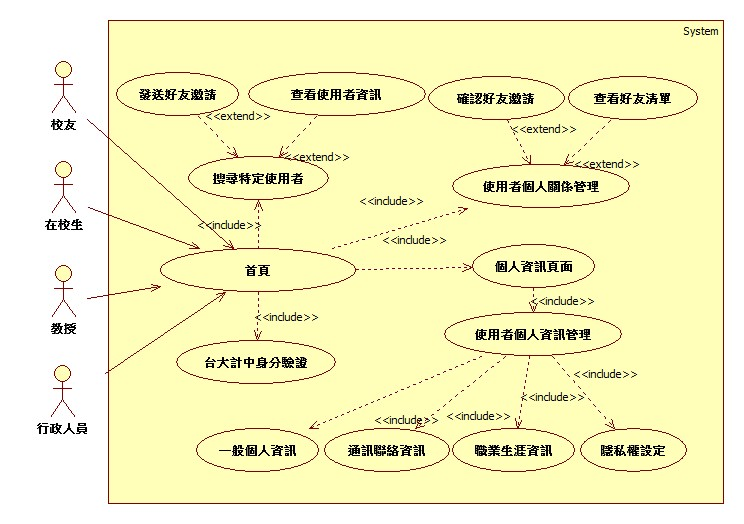
\includegraphics[width=.95\textwidth]{img/useseq/stage1/userProfile.jpg}
\caption{Use Case Diagram -- 使用者資訊管理}
\label{pic:use:userLogin}
\end{figure}

\begin{figure}[H]
\centering
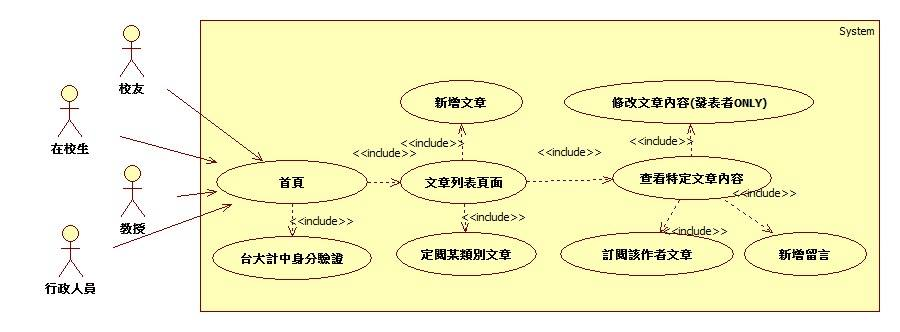
\includegraphics[width=1.05\textwidth]{img/useseq/stage2/useForum.jpg}
\caption{Use Case Diagram -- 文章與留言管理}
\label{pic:use:forum}
\end{figure}


\begin{table}[t]
\centering
\begin{tabular}{ | l | l | l | }
\hline
功能模組 & 功能需求 & 功能範圍 \\ \hline \hline
\multirow{3}{*}{登入模組}
& 輸入身分 & 讓使用者宣稱自己的身分\\
& 身分認證 & 透過計中做身分認證 \\
& 取得token & 回收計中回傳的 token \\ \hline
\multirow{6}{*}{個人資料管理模組}
& 管理公開資料 & 讓使用者維護帳號的公開資訊 \\
& 管理個人聯絡資料& 讓使用者維護帳號的聯絡資料\\
& 職業生涯資料管理& 讓使用者維護職業生涯相關資料 \\
& 隱私權管理$^\star$& 讓使用者管理帳號之公開性選項 \\
& 關係管理$^\star$& 讓使用者管理與其他帳號之間的關係 \\
& 儲存資料異動& 儲存任何使用者新增/修改/刪除之資料 \\ \hline
\multirow{3}{*}{搜尋模組}
& 搜尋特定使用者 & 依照指定學號搜尋符合帳號 \\
& 回傳指定使用者 & 依照指定學號回傳符合條件之帳號 \\ \hline
 \multirow{3}{*}{關係建立模組}
& 傳送使用者好友要求$^\star$ & 由被要求者決定是否成為該用戶之朋友 \\
& 記錄使用者對要求之回應$^\star$ & 提供被要求者回應交友要求 \\
& 記錄使用者之關係狀況 & 儲存所有與其他使用者之間之關係 \\ \hline
\multirow{4}{*}{討論區模組}
& 新增議題 & 讓使用者以自己的帳號新增議題 \\
& 瀏覽議題 & 讓使用者流覽系統中之議題 \\
& 標示議題類別 & 讓使用者清楚了解顯示的議題之標籤 \\
& 管理議題 & 系統管理者確認類別系統正常運作 \\ \hline
\multirow{3}{*}{訂閱模組}
& 訂閱使用者 & 讓使用者關注其他使用者之發文 \\
& 訂閱議題 & 讓使用者關注特定議題的後續發展 \\
& 訂閱議題類別$^\star$ & 讓使用者關注特定議題類別的新增議題 \\ \hline
\multirow{1}{*}{API模組}
& 提供應用編程介面(API) & 使其他服務可藉由 JSON 與本系統互動 \\ \hline
\multirow{2}{*}{行動程式}
& 取得遠端文章資料 & 讓系統透過網路與API互動 \\
& 顯示資料 & 將下載下來的資料呈現給使用者 \\ \hline
\end{tabular}
\caption{功能性需求列表}
\label{req}
\end{table}

\subsection{資料模型}

本節將會介紹本系統所需之資料模型與資料庫設計概念。本系統具有兩個相對複雜且重複性高的功能:「關注」與「留言」;更甚者,此二功能都是未來有可能因為各自牽涉之主體有所異動而需要擴充的部份,因此將此二者予以抽象化就是一項重要的工作。圖~\ref{pic:data:adm} 描述了本專案中的抽象資料模型。可以看到圖~\ref{pic:data:adm} 中的兩個子圖的樣式非常接近,因此更進一步的抽象化是可能的。但是考量到可能之系統規模之後,為了避免過度設計 (over-design) 這邊就不予以進行更進一步之抽象化。另一方面兩圖中灰色的部份是未來可擴充之部分,但是同樣因為系統規模與時程考量而不予實作。

\begin{figure}[h]
\begin{subfigure}[b]{0.5\textwidth}
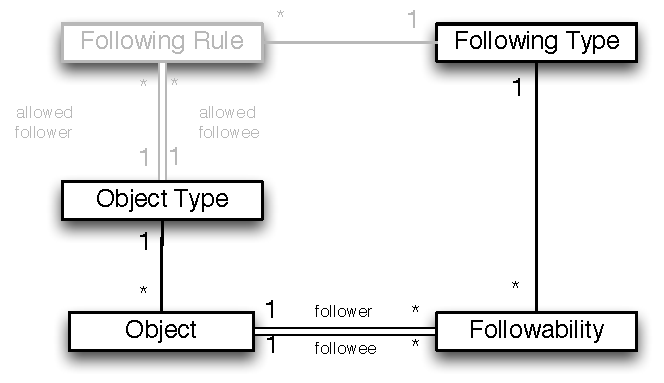
\includegraphics[width=\textwidth]{img/dm1.pdf}
\caption{Followability Model}
\label{pic:data:followability}
\end{subfigure}
\begin{subfigure}[b]{0.5\textwidth}
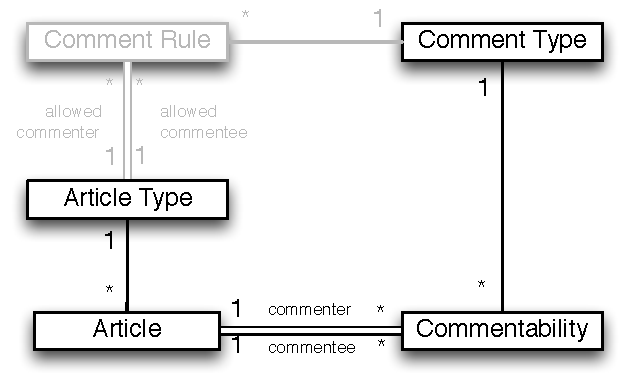
\includegraphics[width=\textwidth]{img/dm2.pdf}
\caption{Commentability Model}
\label{pic:data:commentability}
\end{subfigure}
\caption{Abstract Data Model}
\label{pic:data:adm}
\end{figure}


圖~\ref{pic:data:followability} 描述了廣義的「關注」行為。此行為之概念如下:兩物件 (Object)  可以行成一組關注關係,而根據兩物件與該關注關係之種類可以決定一組實際的系統行為。此模型可以描述例如文章訂閱以及使用者關注等功能。實際上具體的資料模型可以實踐誠如圖~\ref{pic:data:user2user} 與圖~\ref{pic:data:user2article} 中所描述。

圖~\ref{pic:data:commentability} 描述了概念性的「留言」。本系統目前僅有兩種留言模式:預設,以及巢狀留言。預設留言係指使用者可以針對所有非留言之文章進行留言,而巢狀留言則是特指針對現有之留言進行留言。留言行為本身的抽象化是為了未來文章種類或是留言相關功能之擴充所需。實際上具體的資料模型可以實踐誠如圖~\ref{pic:data:comment2article} 中所描述。

\begin{figure}[H]
\centering
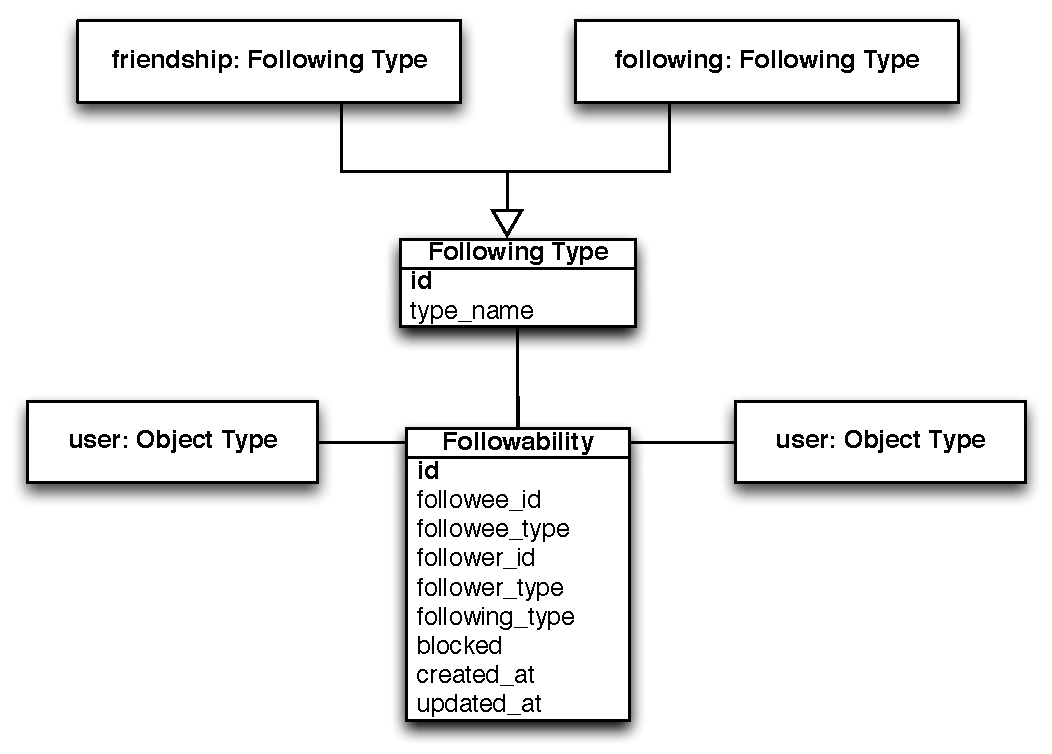
\includegraphics[width=0.75\textwidth]{img/datamodel/user2user.pdf}
\caption{Data Model -- Following and Friendship Model}
\label{pic:data:user2user}
\end{figure}

\begin{figure}[H]
\centering
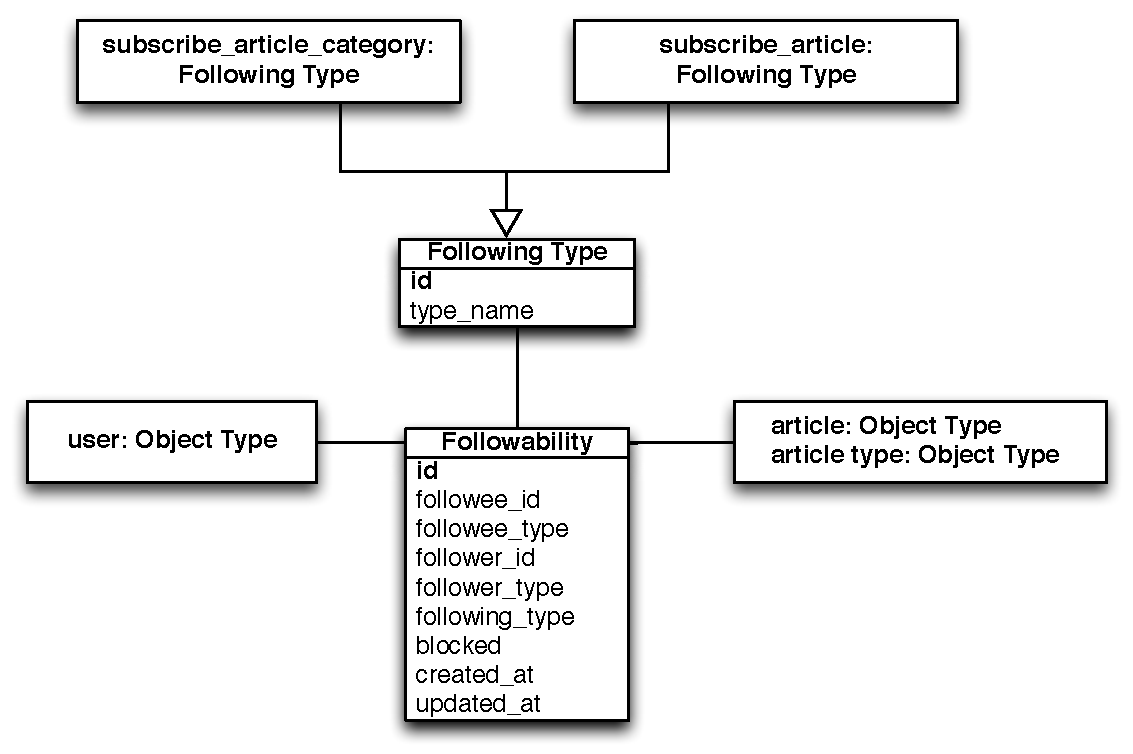
\includegraphics[width=0.75\textwidth]{img/datamodel/user2article.pdf}
\caption{Data Model -- Subscription Model}
\label{pic:data:user2article}
\end{figure}

\begin{figure}[H]
\centering
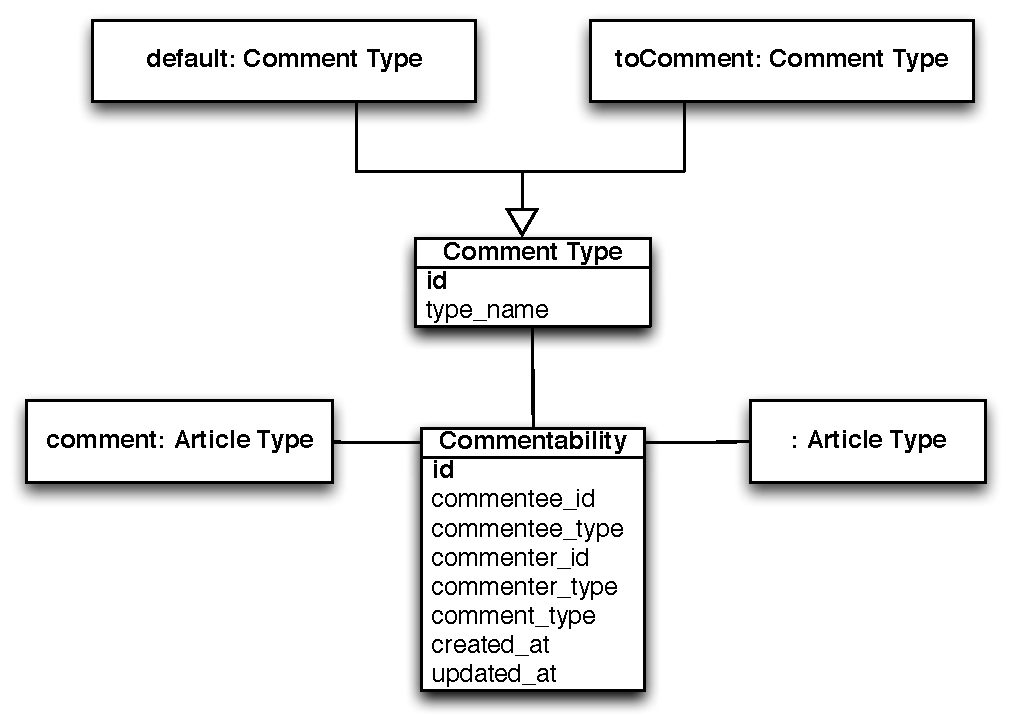
\includegraphics[width=0.75\textwidth]{img/datamodel/comment2article.pdf}
\caption{Data Model -- Comment Model}
\label{pic:data:comment2article}
\end{figure}



%\section{課程心得}
\section{課程心得}
\subsection{郗昀彥 R00725051}

\subsection{郭瀚智 R02725023}

\subsection{鄭立民 R02725041}

於本學期的課程專案中,首先在設計階段學到了許多的UML圖,雖然應用上也只有畫USE CASE跟Sequence而已,但其實許多其他圖的精神也都有包還在內(像是Sequence感覺跟活動流程圖還蠻像的),當然能各種圖都畫出來是最好,也最容易無死角的了解。相信在未來有做專案設計的機會時,這些經驗與知識會有所幫助。

同時在這門課也教了各式設計巧思的Design pattern。雖然沒實際運用過的話,說實在也很難記得。其他還有像是網站資安問題,其中各式各樣的SQL injection讓我最為印象深刻。

本次專案最重要的是,真的體悟到一份專案要管理好實在十分困難,各式各樣的時間不好喬,各式各樣的溝通,加上組員間的能力以及積極度差異,皆會增加做好專案的難易度。
所幸我們有強大的Coding大師們以及組長的積極溝通協調,上山下海全都包,否則產出一份專案當真沒那麼容易。

\subsection{李奕德 B99705021}

在這學期的課程中我學到的Design pattern和Datamodeling令我受益最多,這門課著實地讓我知道我從過去到現在所有寫過的東西都非常的雜亂且狹隘。Android系統的開發上,雖然課堂時間有限所以很緊湊的上了非常多的東西,不過仍然對我們後來再寫手機端時仍然很有幫助。在課堂中所學將我們會用到比較複雜的部份都有帶到,讓開發起來不至於完成不了任何要求。雖然由於時間壓力沒辦法將所有設計都實作,但是仍完成了比較核心的部分。

在這次的project中我們選擇了MVC切割較為清楚的ruby on rails來實作,在製作Android端程式時也將三種不同的面相分成不同的thread去處理以求落實MVC架構。同時,我們盡量在規劃資料模型時讓他具有一定的彈性來使未來需要擴充時不至於完全沒辦法做。

\subsection{張凱涵 B00705027}

\subsection{施淮振 B00705047}

\subsection{倪嘉銘 T02705102}

暑假在家裡選課的時候就對軟體開發這門課程充滿期待,因為在重慶大學的資管系並沒有開設類似的寫程序的課程,然而我對軟體開發還是比較有興趣的,所以很期待這門課程。

在一個學期的學習中,課程的進度顯然要比大陸的的課程快很多,例如我們第一個作業就要求用兩個禮拜完成一個簡單的demo,然而老師在整個過程中都沒有教任何的程式,完全讓學生自己研究。這一點,大陸很難做到,但是其實我還是覺得台灣這樣的教育是非常好的,一方面這樣的方式能夠充分鍛煉學生的自學能力,另一方面也能讓整個課程更加充實,老師能夠講授更多有意義的東西。

在整個學期的過程中,老師邀請的嘉賓從各個方面系統地全面地給我們介紹了軟體開發的各個方面。例如一開始老師就非常強調工具的使用,比如git,這也是在大陸的課程中沒有接觸到的一部分。我能感受的區別就是,台灣的資管系與業界的聯繫要比大陸的資管系課程與業界的練習緊密許多,但是無疑台大這樣的方式能夠讓學生盡早地接觸與業界相關的東西,更能夠適應業界的規則,也能夠讓學生更快地進步。許多嘉賓的講課讓我在軟體開發方面看到了更遠的東西,不再僅僅是將老師要求的功能實現,還有更深遠的程序質量,程序後期的維護,程序的變動,數據模型的合理建構等等。

在project方面,老師要求我們分組做一個校友管理的系統,便是要求我們實作一個程序,我們組所應用的現在漸漸流行的ROR,也讓我接觸到了,業界更新的,更酷的技術,雖然自己在整個開發過程中都出於學習的狀態,並沒有特別多的實作貢獻,但是還是學習到了很多心的東西,收益良多。

有一點比較遺憾的就是之前乜有學習,面向對象的C++和java,所以有些課程並沒有能夠很好地掌握,所以學習效果似乎並沒有那麼好。

總而言之,一個學期的學習還是十分充實的。



\section{工作分配}
本組一共有七個成員,各自負責不同的工作內容而在本專案行進間付出各自的時間和精力。這裡共分成三個階段呈現各位組員的貢獻項目:「前期規劃」意指專案前期的規劃以及分析等工作;「開發期間」則是包含了主要的三個實作階段期間的各個工作項目;「結案階段」條列了專案初步告一段落之後整體的收尾工作項目。

\begin{center}
\begin{table}[!h]
\begin{subtable}{\textwidth}
\begin{tabular}{ | c | c | c | c | c | c | c | c | } \hline
姓名 & 郗昀彥 & 郭瀚智 & 鄭立民 & 李奕德 & 張凱涵 & 施淮振 & 倪嘉銘 \\ \hline \hline
需求分析 & \ci & \ci & \ci & \ci & \ci & \ci & \ci \\ \hline
解決方案 & \ci & \ci & \ci & \ci & \ci & \ci & \ci \\ \hline
專案規劃 & \ci & \ci & & & & & \\ \hline
\end{tabular}
\caption{前期規劃}
\label{charge1}
\end{subtable}
\begin{subtable}{\textwidth}
\begin{tabular}{ | c | c | c | c | c | c | c | c | } \hline
姓名 & 郗昀彥 & 郭瀚智 & 鄭立民 & 李奕德 & 張凱涵 & 施淮振 & 倪嘉銘 \\ \hline \hline
前端設計 & & \ci & & \ci & & & \\ \hline
後端設計 & & \ci & \ci & & & & \\ \hline
資料模型 & \ci & & & & & & \\ \hline
文件設計 & \ci & & & & & & \\ \hline
系統實作 & & \ci & & \ci & \ci & & \ci \\ \hline
文件撰寫 & \ci & & \ci & \ci & \ci & \ci & \ci \\ \hline
系統整合 & & \ci & & & & & \\ \hline
文件整合 & \ci & & & & & \ci & \ci \\ \hline
\end{tabular}
\caption{開發期間}
\label{charge2}
\end{subtable}
\begin{subtable}{\textwidth}
\begin{tabular}{ | c | c | c | c | c | c | c | c | } \hline
姓名 & 郗昀彥 & 郭瀚智 & 鄭立民 & 李奕德 & 張凱涵 & 施淮振 & 倪嘉銘 \\ \hline \hline
系統改進 & & \ci & & \ci & & & \\ \hline
展示規劃 & & & & & \ci & & \ci \\ \hline
報告規劃 & & & \ci & & & \ci & \\ \hline
文件撰寫 & \ci & & & \ci & & & \\ \hline
文件整合 & \ci & & & & & & \\ \hline
\end{tabular}
\caption{結案階段}
\label{charge3}
\end{subtable}
\caption{工作分配}
\label{charge}
\end{table}
\end{center}


\end{document}